\documentclass[final]{beamer}

\newcommand{\trucPleinEcran}[1]{{%
  \setbeamertemplate{navigation symbols}{}%
  \setbeamertemplate{background}{}%
  \setbeamertemplate{background canvas}{%
    \hfill%
    #1
    \hfill%
   }%
   \frame[plain]{}%
}}

\newcommand{\figurePleinEcran}[1]{{%
  \setbeamertemplate{navigation symbols}{}%
  \setbeamertemplate{background}{}%
  \setbeamertemplate{background canvas}{%
    \hfill%
    \includegraphics[width=\paperwidth,height=\paperheight,keepaspectratio]{#1}%
    \hfill%
   }%
   \frame[plain]{}%
}}

%\usepackage{pgfpages}
%\pgfpagesuselayout{2 on 1}[a4paper,border shrink=5mm]

\usepackage{wrapfig}
\usepackage{tikz}
\usetikzlibrary{shapes,arrows}
\usetikzlibrary{fit}					% fitting shapes to coordinates
\usetikzlibrary{backgrounds}	% drawing the background after the foreground
%\usepackage[]{graphicx}
%\usepackage[french,noend]{algorithm2e}
\tikzstyle{background}=[rectangle, fill=gray!10, inner sep=0.2cm, rounded corners=5mm]

\usepackage{fontspec}
\usepackage{xunicode}
\usepackage{xltxtra}
\defaultfontfeatures{Mapping=tex-text}
\setsansfont{Museo Sans}
\setromanfont{Museo}

\mode<presentation> {
  \usetheme{Singapore}
  \setbeamercovered{transparent}
  \AtBeginSection[]{
    \begin{frame}<beamer| handout>[shrink]
      \frametitle{Plan}
      \tableofcontents[sectionstyle=show/shaded,subsectionstyle=show/shaded/hide]
      %\tableofcontents[sectionstyle=show/show,subsectionstyle=show/show/hide]
    \end{frame}}
  \AtBeginSubsection[]{
    \begin{frame}<beamer| handout>[shrink]
      \frametitle{Plan}
      %\tableofcontents[sectionstyle=show/shaded,subsectionstyle=show/shaded/hide]
      \tableofcontents[sectionstyle=show/shaded,subsectionstyle=show/shaded/hide]
    \end{frame}}
}
\setbeamertemplate{navigation symbols}{}

\title{\textsc{Traduction d'OCaml vers une variante de Système F}}
\author{Jonathan Protzenko\\sous la direction de François Pottier}
\date{\today}

\begin{document}

\begin{frame}
  \titlepage
\end{frame}

\section{Introduction}

\subsection{Aperçu du problème}

\begin{frame}{Pourquoi traduire?}
  \begin{columns}
    \column{.5\columnwidth}
      \begin{itemize}
        \item On veut augmenter la confiance dans la chaîne de compilation
        \item ``Well-typed programs can't go wrong'' (Milner)
        \item Le système de types d'OCaml est trop complexe
      \end{itemize}
    \column{.5\columnwidth}
      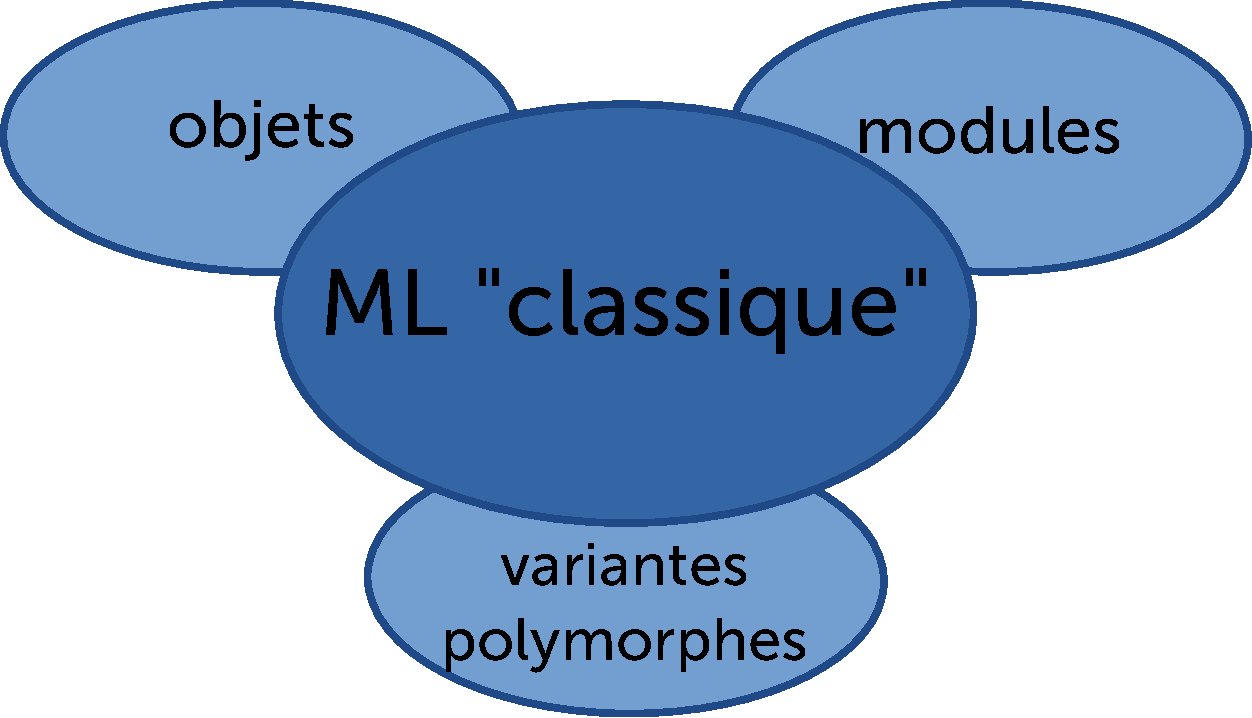
\includegraphics[width=\columnwidth]{ocaml.pdf}
  \end{columns}
  \begin{itemize}
    \item Traduire le programme dans un langage de base
    \item Vérifier le typage \emph{a posteriori}
  \end{itemize}
\end{frame}

\begin{frame}{Objectifs à long terme}
  \begin{itemize}
    \item Fournir un langage intermédiaire pour \emph{effectuer des analyses} et
      compiler plus en avant: expressions \emph{simples}, informations de type
      \emph{riches}.
    \item Augmenter la confiance dans la chaîne de compilation: à défaut de
      prouver la correction du typeur, prouver la cohérence de ses résultats.
    \item Clarifier la sémantique du langage original: quelles sont les
      constructions qui s'expriment bien dans FE+?
  \end{itemize}
\end{frame}

\begin{frame}{Dans les grandes lignes…}
  \begin{center}
    \begin{tikzpicture}
      [node distance = 1cm, auto,
      every node/.style={node distance=3cm},
      pass/.style={shade, shading=axis, rounded rectangle, draw, fill=black!10,
        inner sep=5pt, text width=2cm,
        text badly centered, minimum height=1.2cm, font=\bfseries\scriptsize\sffamily},
      tool/.style={rectangle, draw, thick, fill=black!10, inner sep=5pt, text
        width=1.5cm,
        text badly centered, minimum height=.8cm, font=\bfseries\scriptsize\sffamily}] 
      % Place nodes
      \node [pass] (solve) {Résolution de contraintes};
      \node [left of=solve, node distance=3.5cm] (phantom) {};
      \node [pass, above of=phantom, node distance=1cm] (gen) {Génération de contraintes};
      \node [pass, dashed, below of=phantom, node distance=1cm] (gen2) {Autre langage de surface};
      \node [pass, right of=solve, node distance=3.5cm] (camlx) {AST annoté (CamlX)};
      \node [pass, below of=camlx] (fe) {Langage Core (Système FE+)};
      \node [tool, left of=fe] (typecheck) {Type-checking};
      %\node [block, below of=solve] (unify) {Moteur d'unification};
      % Draw edges
      \draw [->, thick] (gen) -- (solve);
      \draw [->, thick, dashed] (gen2) -- (solve);
      \draw [->, thick] (solve) -- (camlx);
      \draw [->, thick] (camlx) -- (fe);
      \draw [->, thick] (typecheck) -- (fe);
      %\path [line, <->] (unify) -- (solve);
      \begin{pgfonlayer}{background}
        \node [background, fit=(gen) (gen2) (solve), pin=-100:Inférence] {};
        \node [background, fit=(camlx) (fe), pin=80:Traduction] {};
      \end{pgfonlayer}

    \end{tikzpicture}
  \end{center}
  \footnotesize Le processus se découpe en deux parties~: génération/résolution de
  contraintes, et traductions jusqu'à Système FE+.
\end{frame}

\subsection{Contributions}

\begin{frame}{Trois grands axes de travail}
  \begin{columns}
    \column{.5\columnwidth}
      \begin{itemize}
        \item Récrire un système d'inférence par contraintes, et l'adapter pour
          donner un \emph{AST annoté}.
        \item Élaborer un processus de traduction d'un fragment d'OCaml vers un
          langage minimaliste
        \item Concevoir le système de types qui permet de justifier le comportement
          d'OCaml
      \end{itemize}
    \column{.5\columnwidth}
      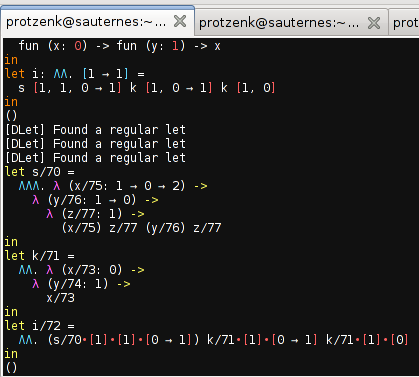
\includegraphics[width=\columnwidth]{screen1.png}
  \end{columns}
\end{frame}

\section{Décoration d'ASTs}

\subsection{Le cœur du problème}

\begin{frame}{Présentation de l'inférence par contraintes}
  \begin{itemize}
    \item Nouvelle présentation d'un algorithme <<~classique~>>
    \item Séparation claire et élégante entre génération et résolution
    \item 
  \end{itemize}<++>
\end{frame}

\begin{frame}{<++>}
<++>
\end{frame}

\begin{frame}{<++>}
<++>
\end{frame}

\begin{frame}{<++>}
<++>
\end{frame}

\begin{frame}{<++>}
<++>
\end{frame}

\begin{frame}{<++>}
<++>
\end{frame}

\begin{frame}{<++>}
<++>
\end{frame}

\begin{frame}{<++>}
<++>
\end{frame}

\begin{frame}{<++>}
<++>
\end{frame}

\begin{frame}{<++>}
<++>
\end{frame}

\begin{frame}{<++>}
<++>
\end{frame}

\begin{frame}{<++>}
<++>
\end{frame}

\begin{frame}{<++>}
<++>
\end{frame}

\begin{frame}{<++>}
<++>
\end{frame}

\begin{frame}{<++>}
<++>
\end{frame}

\begin{frame}{<++>}
<++>
\end{frame}

\begin{frame}{<++>}
<++>
\end{frame}

\end{document}
